\section{花苗分类问题}
该问题来自于kaggle的Plant Seedlings Classification竞赛。给定的13类花苗(有枝干,树叶,无花)的四千余张彩色图片用于训练、构建模型。其数据基本情况如下
\begin{center}
\begin{tabular}{ccc}
\toprule[2pt]
序号 & 种类 & 样本数量 \\ 
\midrule[1pt]
1 & Black-grass & 263 \\ 
2 & Charlock & 390 \\ 
3 & Cleavers & 287 \\ 
4 & Common Chickweed & 611 \\ 
5 & Common wheat & 221 \\ 
6 & Fat Hen & 475 \\ 
7 & Loose Silky-bent & 654 \\ 
8 & Maize & 221 \\  
9 & Scentless Mayweed & 516 \\ 
10 & Shepherds Purse & 231 \\ 
11 & Small-flowered Cranesbill & 496 \\ 
12 & Sugar beet & 385 \\ 
\midrule[1pt]
总和 & -- & 4750\\
\bottomrule[2pt]
\end{tabular} 
\end{center}
而且每一张的图片大小都有可能不同。每一类的图像的例子如下
\begin{center}
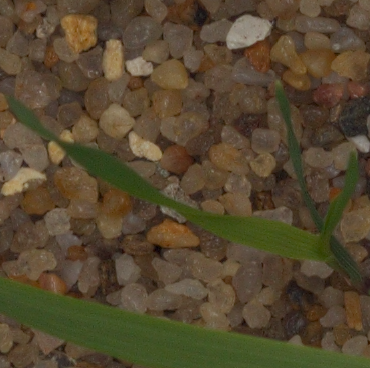
\includegraphics[width=30mm,height=30mm]{../figures/Black-grass_1af1eddd3.png} 
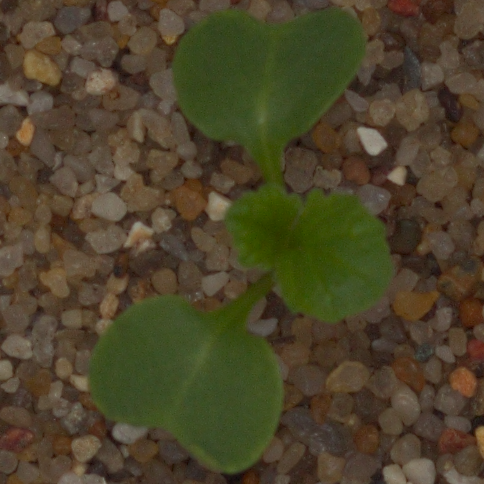
\includegraphics[width=30mm,height=30mm]{../figures/Charlock_0a7e1ca41.png} 	
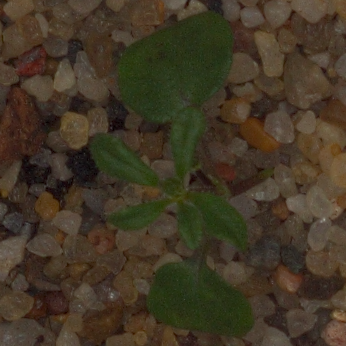
\includegraphics[width=30mm,height=30mm]{../figures/Cleavers_0a1e622bc.png} 	\\
Black-grass,Charlock,Cleavers
\end{center}
\begin{center}
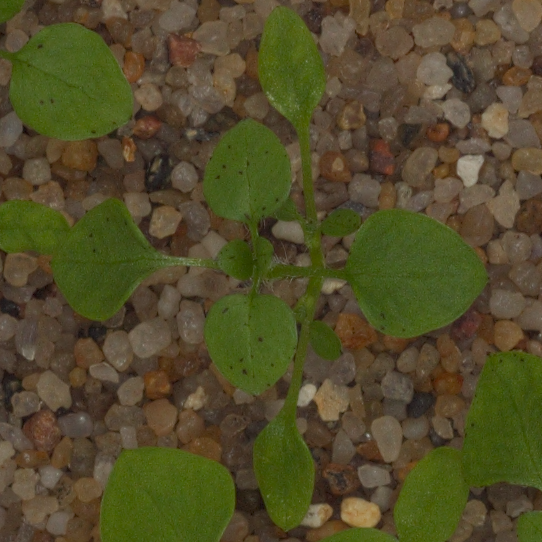
\includegraphics[width=30mm,height=30mm]{../figures/Common_Chickweed_0a1c68ef9.png} 	
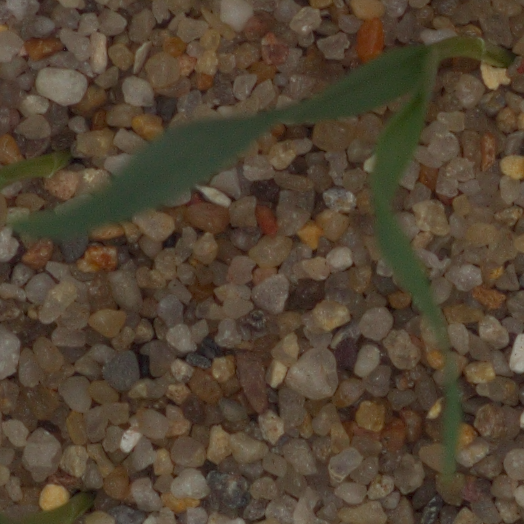
\includegraphics[width=30mm,height=30mm]{../figures/Common_wheat_6dfb9a152.png} 	
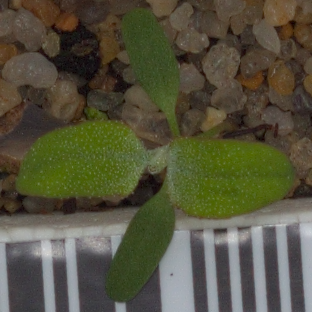
\includegraphics[width=30mm,height=30mm]{../figures/Fat_Hen_0eeb0c7c1.png} 	\\
Common Chickweed,Common wheat,Fat Hen
\end{center}
\begin{center}
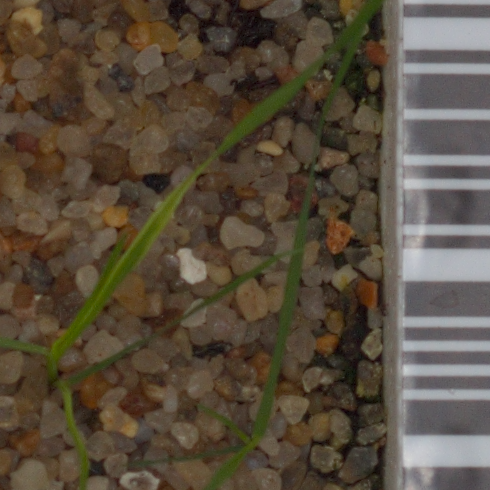
\includegraphics[width=30mm,height=30mm]{../figures/Loose_Silky-bent_3cac767c2.png} 	
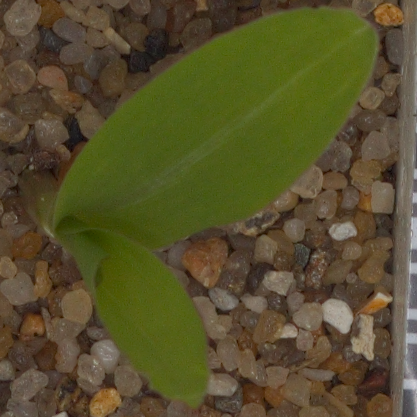
\includegraphics[width=30mm,height=30mm]{../figures/Maize_1d21b25f9.png}	
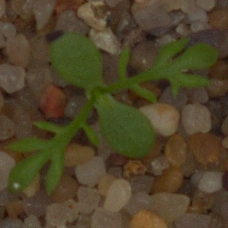
\includegraphics[width=30mm,height=30mm]{../figures/Scentless_Mayweed_0ae9acf83.png} 	\\
Loose Silky-bent,Maize,Scentless Mayweed
\end{center}
\begin{center}
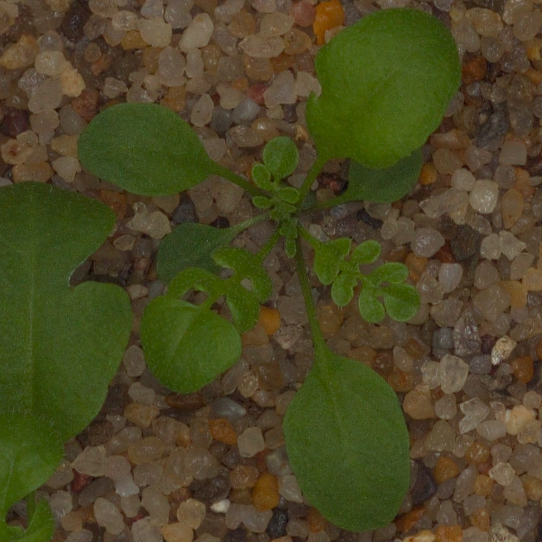
\includegraphics[width=30mm,height=30mm]{../figures/Shepherds_Purse_0bef4ae08.png} 	
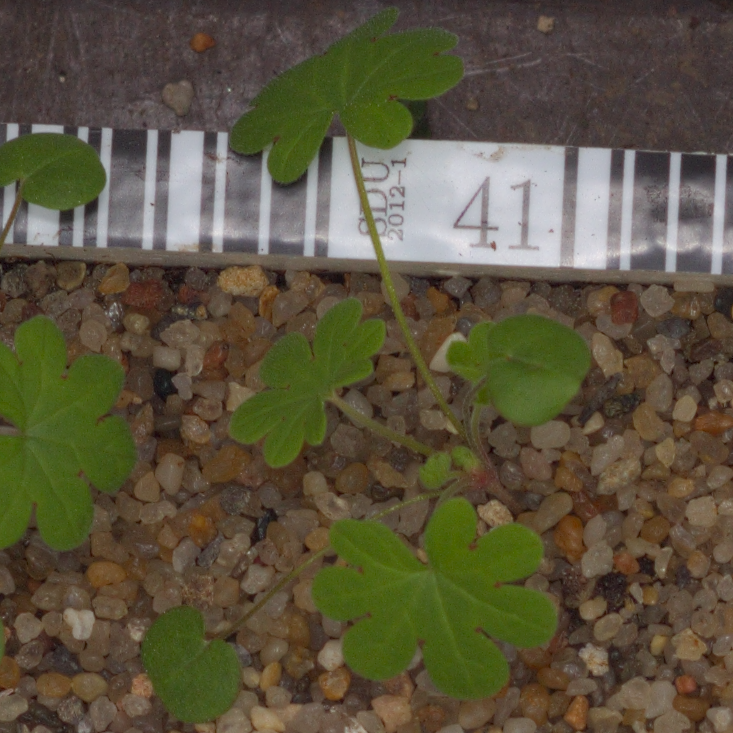
\includegraphics[width=30mm,height=30mm]{../figures/Small-flowered_Cranesbill_0e7f05ec0.png} 	
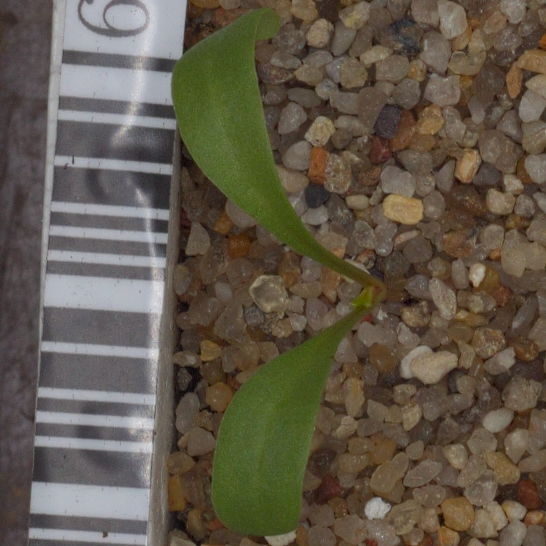
\includegraphics[width=30mm,height=30mm]{../figures/Sugar_beet_1bdfd2206.png} 	\\
Shepherds Purse,Small-flowered Cranesbill,Sugar beet
\end{center}

由于所涉及到的数据为彩色图像,而花苗的特征为绿色,故考虑使用opencv的方法,通过建立掩膜筛选出花苗的图像,进而将彩色图像转化为灰度图像或二值图像,从而达到降维的目的。而即使降维之后,为了确保图像失真不大,所以至少将图像转化为$64\times 64$的灰度图像矩阵。若考虑直接采用Logistic、SVM或决策树方法,则需要将$64\times 64$的灰度图像矩阵拉伸为$4096\times 1$的图像,然而假设用全部的数据进行训练,也只有4750个样本,训练时极容易导致过拟合,但是,考虑集成学习的方法或是带dropout的BP神经网络可以一定程度上防止过拟合。考虑到为涉及图像的分类问题,可以采用卷积神经网络(CNN)。由于是13类的分类问题,且样本数较少,可以进一步考虑在用SVM、Logistic或决策树方法来替代神经网络最后的softmax层,或许能起到更好的效果。